\chapter{Introduction}
\label{chapter:intro}

{\color{red} TODO: hyphenation}

{\color{red} TODO: spell check}

Most people nowadays are familiar with \textit{projection}, the act of transferring images from film or computer memory onto screens in cinemas and classrooms. But while those screens are made specifically for being projected onto, this is not the case for other objects, for example building façades. The geometry and material properties of these objects deform projected images and change their appearance. This is why projecting them is not enough -- they first need to be edited (\textit{mapped}) in a way that their final appearance is what we expect. Projecting onto arbitrary objects in such a way is called \textit{projection mapping} and it is the main topic of this thesis.

\begin{figure}[ht]
    \centering
    \begin{subfigure}[b]{0.49\textwidth}
        \centering
        \includegraphics[width=\textwidth]{images/01-sydney_opera_house_night-edit.jpg}
        \caption{}
        %\label{}
    \end{subfigure}
    \hfill
    \begin{subfigure}[b]{0.49\textwidth}
        \centering
        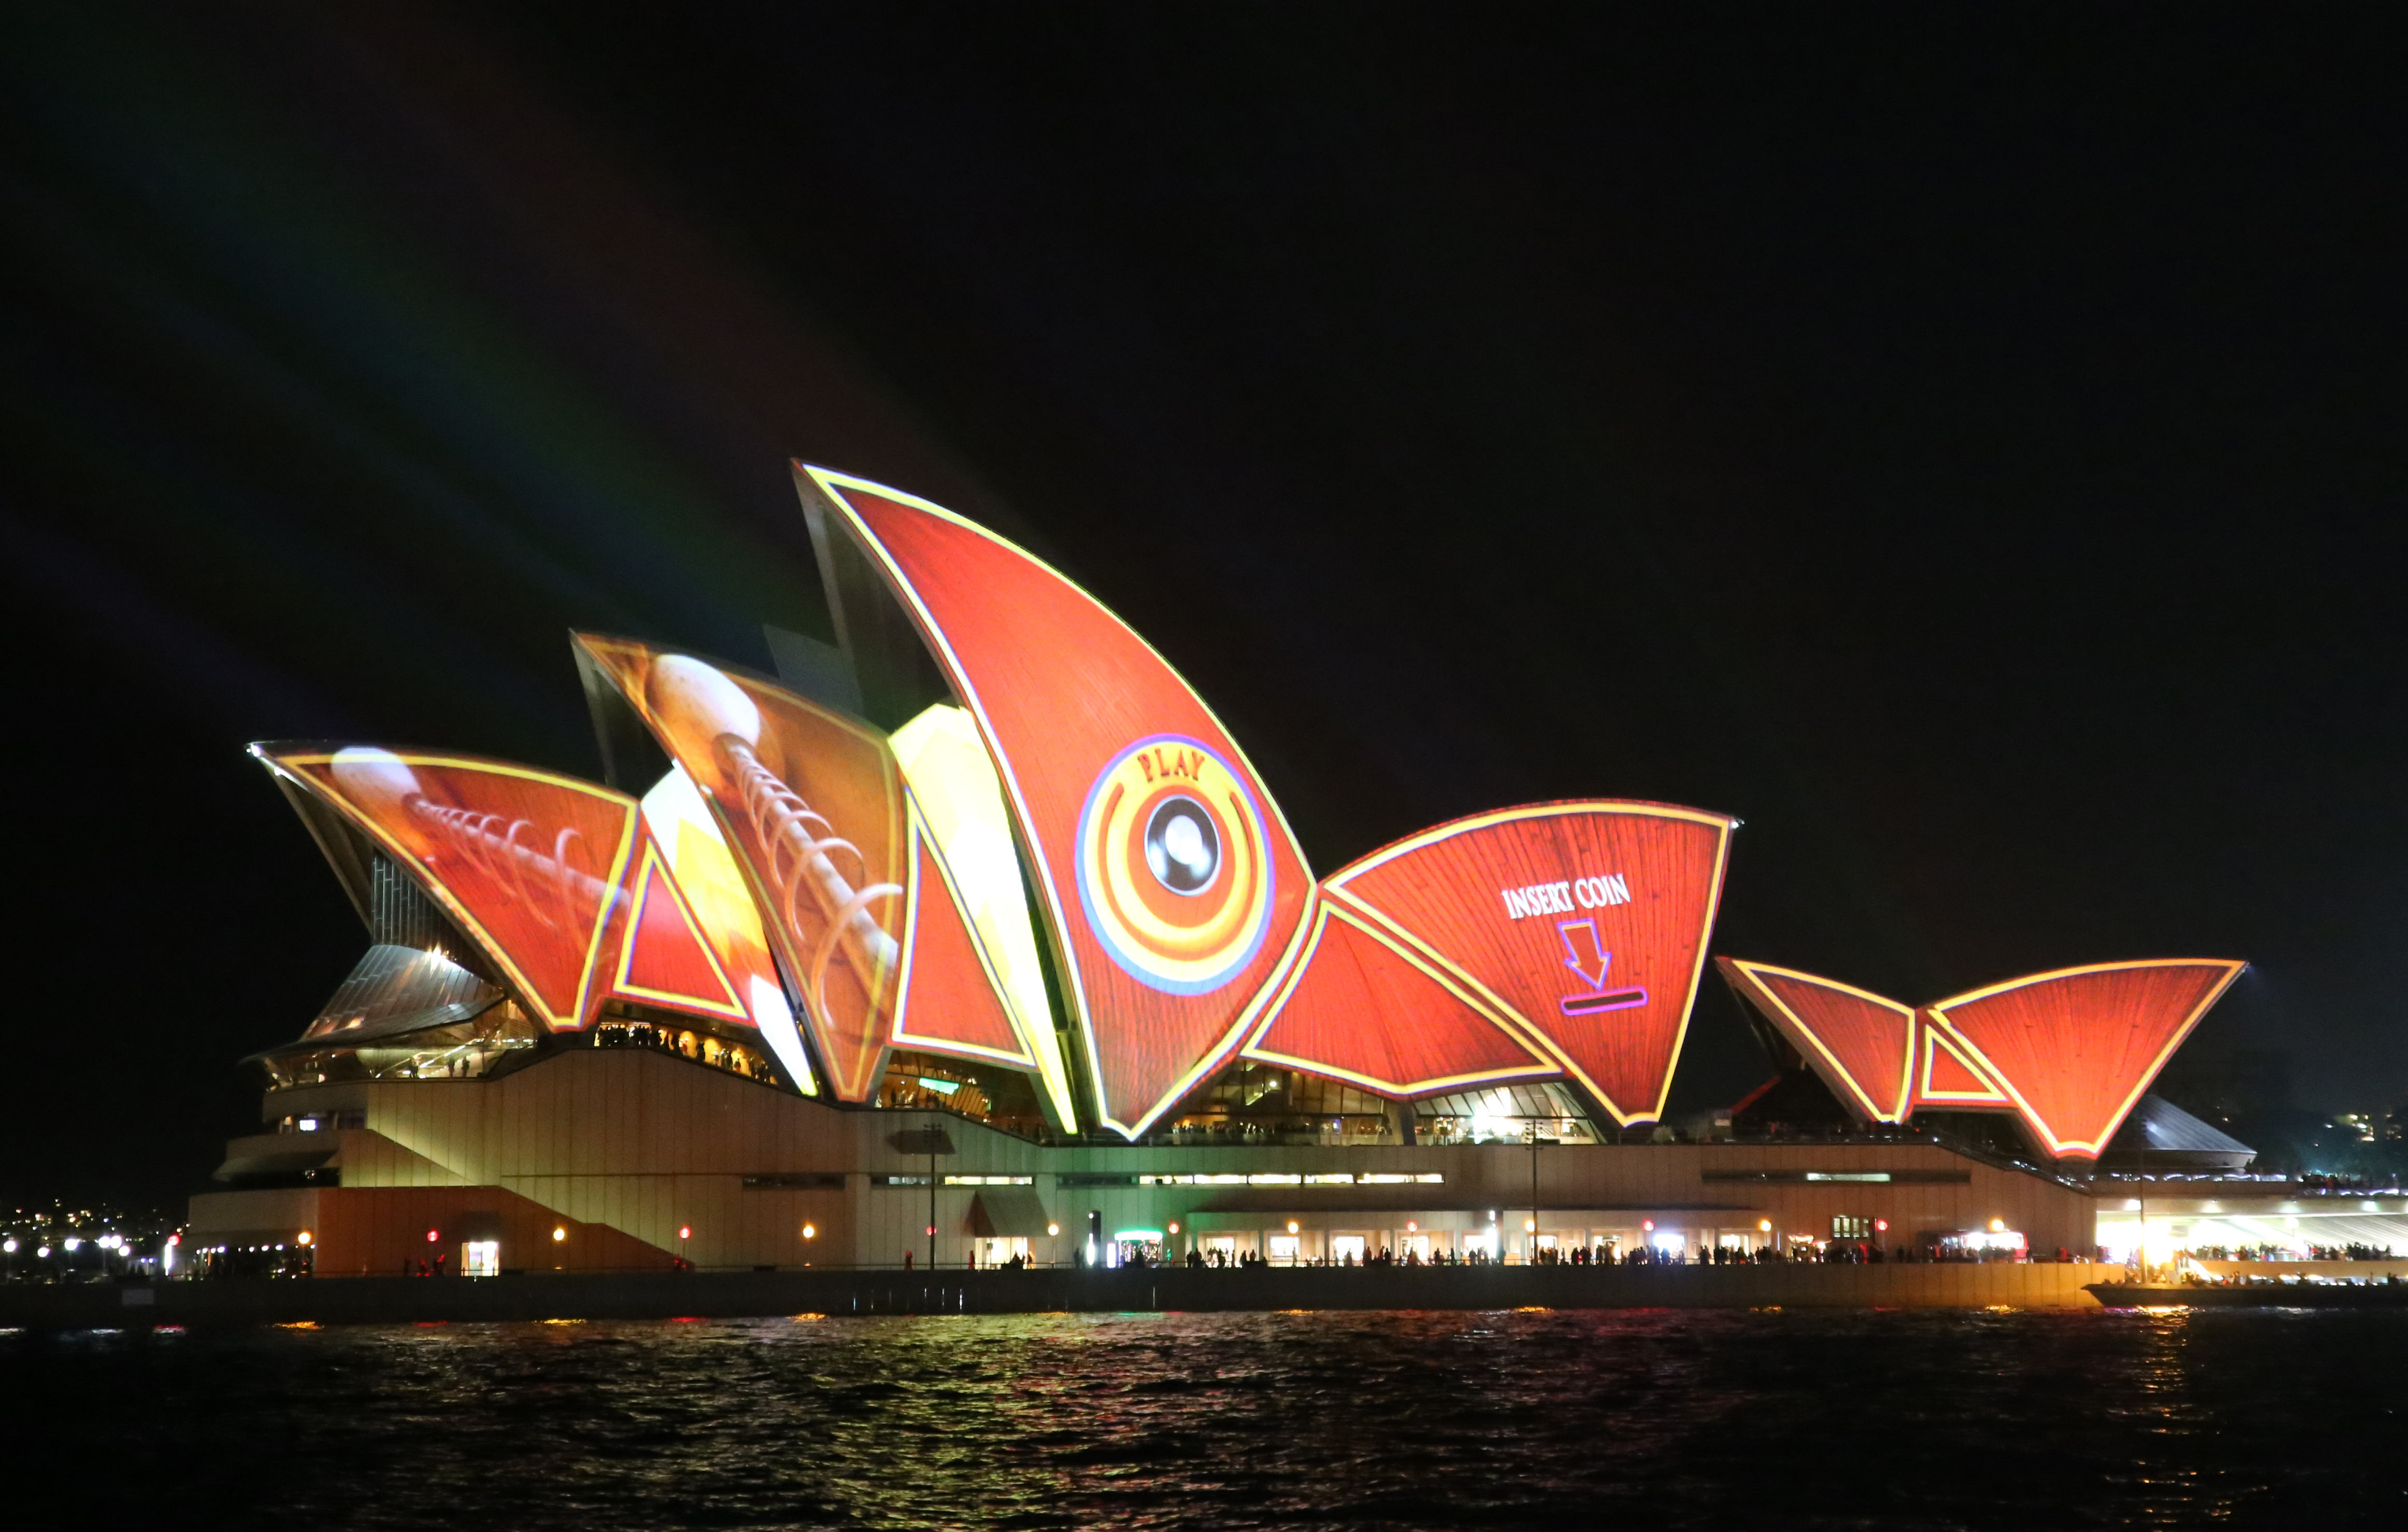
\includegraphics[width=\textwidth]{images/01-sydney_opera_house_projection1.jpg}
        \caption{Source: \citet{ImageProjectionMappingExampleSydney}}
        %\label{}
    \end{subfigure}
    \caption{The Sydney Opera House with (b) and without (a) projection mapping.}
    \label{fig:intro_example_sydney}
\end{figure}

According to \citet*{WikiHauntedMansion}, one of the first uses of projection mapping (also sometimes called \textit{video mapping} or \textit{spatial augmented reality}) was in the character of Madame Leota in The Haunted Mansion Disneyland ride which opened in 1969. There, a video of a human face was projected onto a static head (see gig. \ref{fig:intro_example_leota}). Nowadays, projection mapping has become widespread. It is used to augment reality by artists from all over the world in galleries, museums and outdoor spaces. One prominent example is projection mapping on buildings (see figure \ref{fig:intro_example_sydney}) which is done in cities during festivals and on other special occasions.

\begin{figure}[ht]
    \centering
    \begin{subfigure}{0.6\textwidth}
        \centering
        \includegraphics[width=\textwidth]{images/01-Leota.jpg}
        \caption{}
        \label{fig:intro_example_leota-full}
    \end{subfigure}
    \hfill
    \begin{subfigure}{0.39\textwidth}
        \centering
        \begin{subfigure}{\textwidth}
            \centering
            \includegraphics[width=\textwidth]{images/01-Leota-no_head.jpg}
            \caption{}
            \label{fig:intro_example_leota-scene}
        \end{subfigure}
        
        \begin{subfigure}{\textwidth}
            \centering
            \includegraphics[width=\textwidth]{images/01-Leota-only_head.jpg}
            \caption{}
            \label{fig:intro_example_leota-head}
        \end{subfigure}
    \end{subfigure}
    \caption{The character of Madame Leota in Disneyland's Haunted Mansion ride is one of the earliest examples of projection mapping. A video of her face is projected onto a round disk to give an illusion of a head inside a crystal ball. Included is our simplified decomposition of the scene (\ref{fig:intro_example_leota-full}) into background (\ref{fig:intro_example_leota-scene}) and projection image (\ref{fig:intro_example_leota-head})}
    \label{fig:intro_example_leota}
\end{figure}

Let us now briefly describe what projection mapping entails and which of its problems we aim to address in this thesis.

\section{Problem Setting}
\label{section:intro-problem_setting}

Simply put, projection mapping is projecting onto surfaces that are not primarily intended for projection and often have complex texture or geometry. In this thesis, we formulate the projection mapping problem as follows:

\begin{enumerate}
    \item We begin with a scene, for example fig. \ref{fig:intro_example_leota-scene}
    \item We choose what we would want it to look like after projection (i.e the \textit{desired appearance}), for example \ref{fig:intro_example_leota-full}
    \item The task is to create a \textit{compensated projection image} that will look like our desired appearance when projected onto our scene, for example fig. \ref{fig:intro_example_leota-head}
    \item We project the compensated image
\end{enumerate}

There is a wide body of research focusing on creating such compensated images automatically given a scene and a desired appearance. In one of the earliest papers of the field, \citet*{Grossberg2004} project a series of special calibration images onto a scene and capture their appearance using a camera. Using these \textit{camera images}, they are able to estimate how each pixel of the projection influences the appearance of that particular scene. Once this calibration is ready, they are able to quickly compute compensation images on the fly and only project the compensations (see fig. \ref{fig:intro_grossberg} for an example). The combination of a projector and a camera is common in projection mapping and such systems are called \textit{projector-camera systems} (see fig. \ref{fig:intro_procam}).

\begin{figure}[ht]
    \centering    
    \begin{subfigure}{0.8\textwidth}
        \centering
        \begin{subfigure}{0.3\textwidth}
            \centering
            \includegraphics[width=\textwidth]{images/01-desired_appearance.png}
            \caption{Desired appearance}
            \label{fig:intro_grossberg-desired_appearance}
        \end{subfigure}
        \hfill
        \begin{subfigure}{0.3\textwidth}
            \centering
            \includegraphics[width=\textwidth]{images/01-background.png}
            \caption{Background}
            \label{fig:intro_grossberg-background}
        \end{subfigure}
        \hfill
        \begin{subfigure}{0.3\textwidth}
            \centering
            \includegraphics[width=\textwidth]{images/01-uncompensated.png}
            \caption{\ref{fig:intro_grossberg-desired_appearance} projected onto \ref{fig:intro_grossberg-background}}
            \label{fig:intro_grossberg-uncompensated}
        \end{subfigure}
        
        \begin{subfigure}{0.3\textwidth}
            \centering
            \includegraphics[width=\textwidth]{images/01-compensation_image.png}
            \caption{Compensated projection image}
            \label{fig:intro_grossberg-compensation}
        \end{subfigure}
        \hfill
        \begin{subfigure}{0.3\textwidth}
            \centering
            \includegraphics[width=\textwidth]{images/01-new_appearance.png}
            \caption{\ref{fig:intro_grossberg-compensation} projected onto \ref{fig:intro_grossberg-background}}
            \label{fig:intro_grossberg-new_appearance}
        \end{subfigure}
    \end{subfigure}
    \caption{Automatic projection mapping as presented in \citet{Grossberg2004}}
    \label{fig:intro_grossberg}
\end{figure}

\begin{figure}[ht]
    \centering
    \includegraphics[width=0.6\textwidth]{images/01-procam.png}
    \caption{Projector-camera system from \citet{Grossberg2004}}
    \label{fig:intro_procam}
\end{figure}

Since then, there have been many advances in the field, the summary of which can be found in a state-of-the-art report by \citet*{Grundhofer2018}. The latest projector-camera systems are able to calibrate themselves automatically after they are placed in a scene, re-calibrate when scene illumination changes, or when objects in the scene are transformed, both rigidly (i.e. without deformation) and non-rigidly. Some can do this in real time. Because of the sheer complexity of general projection mapping, however, no single method can do all these things at once. For example, methods that handle non-rigid transformations will often rely on object tracking which requires the object to have markers on it. Such methods might also break when illumination changes significantly.

There is, however, one fundamental characteristic that all current projection mapping methods share. When computing the compensated projection image, they match the camera image with the desired appearance pixel by pixel. Explicitly, their goal is the following:

\begin{equation}
    \label{eq:projection_mapping-per_pixel}
    \min_p \sum_{i=1}^{m \cdot n} || x(p)_{(i)} - y_{(i)} ||
\end{equation}

where \(p\) is the projector image, \(x(p) \in \mathbb{R}^{m \times n}\) is the camera image when \(p\) is projected, \(y\) is the desired appearance and \((i)\) selects the \(i\)-th pixel of an image. Note that \(x\) is determined by the projector and the scene.

This approach is limited by projector hardware. Every projector has finite brightness which means that pixels of the camera image cannot be made arbitrarily bright (\(x(p) \leq c;\; \forall p\)). In scenes with external illumination, it is also impossible to make pixels of the camera image arbitrarily dark since projectors only add light and do not subtract it (\(x(p) \geq 0;\; \forall p\)). In the notation introduced above this mean that for any projector image \(p\)

\begin{equation}
    \label{eq:projection_mapping-limitations}
    \forall i:\; 0 \leq x(p)_{(i)} \leq c_{(i)}
\end{equation}

where \(c\) is a constant vector that depends on the projector and the scene.

For every projector and scene, we can therefore find an image \(y\) whose pixels are too dark or too bright such that they cannot be mapped using the recipe in eq. \ref{eq:projection_mapping-per_pixel}:

\begin{equation}
    \label{eq:projection_mapping-hard_image}
    \exists i:\; y_{(i)} < 0 \lor y_{(i)} > c_{(i)}
\end{equation}

Figure \ref{fig:intro_pixels_vs_stats} shows images \(y_1\) and \(y_2\) where the former fulfills eq. \ref{eq:projection_mapping-hard_image} for a given projector and scene and is thus impossible to map while the latter is the opposite.

\begin{figure}[ht]
    \centering    
    \begin{subfigure}{\textwidth}
        \centering
        \begin{subfigure}{0.2\textwidth}
            \centering
            \includegraphics[width=\textwidth]{images/01-pixels_vs_stats-pixels_target.jpg}
            \caption*{\(y_1\)}
            \label{fig:intro_pixels_vs_stats-pixels_target}
        \end{subfigure}
        \hfill
        \begin{subfigure}{0.2\textwidth}
            \centering
            \includegraphics[width=\textwidth]{images/01-pixels_vs_stats-bg.jpg}
            \caption*{Scene}
            \label{fig:intro_pixels_vs_stats-pixels_bg}
        \end{subfigure}
        \hfill
        \begin{subfigure}{0.2\textwidth}
            \centering
            \includegraphics[width=\textwidth]{images/01-pixels_vs_stats-pixels_opt.jpg}
            \caption*{\(p_1\)}
            \label{fig:intro_pixels_vs_stats-pixels_opt}
        \end{subfigure}
        \hfill
        \begin{subfigure}{0.2\textwidth}
            \centering
            \includegraphics[width=\textwidth]{images/01-pixels_vs_stats-pixels_proj.jpg}
            \caption*{\(x(p_1)\)}
            \label{fig:intro_pixels_vs_stats-pixels_proj}
        \end{subfigure}
        
        \begin{subfigure}{0.2\textwidth}
            \centering
            \includegraphics[width=\textwidth]{images/01-pixels_vs_stats-stats_target.jpg}
            \caption*{\(y_2\)}
            \label{fig:intro_pixels_vs_stats-stats_target}
        \end{subfigure}
        \hfill
        \begin{subfigure}{0.2\textwidth}
            \centering
            \includegraphics[width=\textwidth]{images/01-pixels_vs_stats-bg.jpg}
            \caption*{Scene}
            \label{fig:intro_pixels_vs_stats-stats_bg}
        \end{subfigure}
        \hfill
        \begin{subfigure}{0.2\textwidth}
            \centering
            \includegraphics[width=\textwidth]{images/01-pixels_vs_stats-stats_opt.jpg}
            \caption*{\(p_2\)}
            \label{fig:intro_pixels_vs_stats-stats_opt}
        \end{subfigure}
        \hfill
        \begin{subfigure}{0.2\textwidth}
            \centering
            \includegraphics[width=\textwidth]{images/01-pixels_vs_stats-stats_proj.jpg}
            \caption*{\(x(p_2)\)}
            \label{fig:intro_pixels_vs_stats-stats_proj}
        \end{subfigure}
    \end{subfigure}
    \caption{Two examples of projection mapping: failure (top row) and success (bottom row). Both examples follow the formula in eq. \ref{eq:projection_mapping-per_pixel} and both have the same scene (background) and projector. The only difference is the desired appearance. Leftmost column shows the desired appearance, middle-left column shows the background, middle-right column shows the compensated projection image and rightmost column shows the camera image.}
    \label{fig:intro_pixels_vs_stats}
\end{figure}

In this thesis, we reformulate the projection mapping recipe in eq. \ref{eq:projection_mapping-per_pixel} to overcome this limitation and present a technique that uses our new recipe to achieve results that have not been achieved before.

\section{Key Idea}
\label{section:intro-key_idea}

{\color{red} TODO: overall, maybe skip the deeper theory here. Only present what's absolutely crucial to understanding the key idea and do that on a high level. Explain the rest in the Background section. Don't do forward references, but depth references instead... Example: Why do you explain parametric synthesis here quite in-depth, but non-parametric synthesis not at all? It's fine to handwave here if you do the depth referencing thing.}

{\color{red} TODO: mention the Texture Hypothesis by Julesz (texture is defined by 2nd order co-occuring stationary statistics) here}

Textures (e.g. an image of a stony beach) have the interesting property that when their features (e.g. individual stones) are shuffled, the texture still looks the same. For example, \citet*{Julesz1995} defines textures as classes of images that cannot be discriminated in preattentive vision. These images are not the same pixel by pixel, but they \textit{look} the same when we glance over them.

{\color{red} TODO: figure of the main idea}

We present a method for projection mapping textures, using their properties to achieve high-quality results as follows:

\begin{itemize}
    \item We assume a texture which is difficult to project-map onto a given scene because of brightness limitations of the projector
    \item Out of all possible realizations of that texture, we find the one which minimizes the number of pixels which the projector would struggle to reproduce
    \item We find the appropriate compensated projection image for it
\end{itemize}

A separate research field is dedicated to generating different realizations of the same texture, a task which came to be called \textit{texture synthesis}. \citet*{Raad2018} present a state-of-the-art report of texture synthesis methods. Some of these methods derive a statistical representation of textures such that if two pictures share that representation, they are the same texture, even if their pixel values are different. Here are some examples of what is meant by statistical representation:

\begin{itemize}
    \item Pixel values (this is too restrictive because in this case all texture classes only contain a single image)
    \item Average color (this is too loose because in this case each texture class would contain e.g. a constant image of that color)
    \item Power spectrum (a better representation which works well for textures with tiny features and is used for texture synthesis in \citet*{Galerne2011})
    \item Gram matrices of feature activations of a convolutional neural network (a complex representation presented by \citet*{Gatys2015} which significantly increased the quality of texture synthesis and spurred a wave of new research in the area, including this thesis)
\end{itemize}

{\color{red} TODO: figure to illustrate statistical representations}

We build on these statistics-based synthesis methods and reformulate the goal of projection mapping as follows:

\begin{equation}
    \label{eq:projection_mapping-statistics}
    f(X) = f(Y)
\end{equation}

where \(X,Y \in \mathbb{R}^{n \times m}\) are again the camera image and desired appearance, respectively, and \(f\) is a function that assigns a statistical representation to an image.

An important observation is that images that have equal pixel values also share their statistical representation. Therefore, this formulation of the projection mapping problem is strictly more powerful than the pixel-based one if the following conditions hold:

\begin{enumerate}
    \item \(f\) describes textures well -- all textures that look the same share the same \(f\)-value and no two textures that look different share the same \(f\)-value
    \item An algorithm exists that can find such \(X\) and \(Y\)
\end{enumerate}

We now specify what the contributions of this thesis are.

\section{Contributions}
\label{section:intro-contributions}

Solving both the problem of texture synthesis and projection mapping is very challenging. In this thesis, we therefore focus mainly on showing that by combining existing methods from both fields, interesting results can be achieved that have not been achieved before.

Our contributions are the following:

\begin{itemize}
    \item We implement our proposed method as outlined in section \ref{section:intro-key_idea} in PyTorch as an optimization loop. No projector and camera hardware is involved.
    \item We guide the reader through three experiments whose aim is to evaluate the proposed method and compare it to current pixel-based approaches. Here is a summary of their conclusions:
    \begin{enumerate}
        \item In a simplified scenario without complex geometry or global illumination effects, our optimizer is able to generate a texture that is both part of a given texture class (as defined by existing texture synthesis methods) and adapted to fit the given scene well when projected.
        \item In a simplified scenario, our method outperforms current pixel-based methods in certain challenging conditions as expected.
        \item Our method works just as well in scenarios with complex geometry and global illumination effects as it does in simplified scenarios.
    \end{enumerate}
\end{itemize}

{\color{red} TODO: single target-scene-compensation-appearance results teaser with a single, well described point}

\section{Thesis Structure}
\label{section:intro-thesis_structure}

This thesis is organized as follows. In chapter \ref{chapter:background}, we provide an overview of the state of the art in projection mapping and texture synthesis and explain in detail the methods which we build on later on. In chapter \ref{chapter:methods}, we describe our method, its implementation and how each of the three experiments is constructed. In chapter \ref{chapter:results}, we present the results of the experiments and analyze them. Lastly, in chapter \ref{chapter:conclusions} we conclude the thesis and discuss future work.
